\documentclass[12pt,fleqn]{article}\usepackage{../../common}
\begin{document}
Materyel Mekaniği - 2

Sonsuz Küçük (Infinitesimal) Gerilme Tensörü

Green gerilme tensörünü gördük, kuvvetli bir yaklaşım ama bizim daha çok
kullanacağımız şimdi anlatacağımız. Niye? Çünkü Green tensoru sonlu değişimler
için geçerli ama çoğu uygulamada bize lazım olan çok ufak yamulmalar. Ufak
değişimler derken, (3) formülünden hareketle, oradaki en son terimi hatırlarsak,
çok ufak yamulmalar için $\nabla u^T \nabla u << \nabla u$ olur, yani ufak
değişimlerde o karesel işlem $\nabla u$'dan daha ufak sonuç verir. O zaman belli
durumlarda son terim yaklaşık sıfır kabul edilebilir, $\nabla u^T \nabla u
\approx 0$. O zaman Green tensörü bu durumlarda yaklaşık olarak alttaki gibi
olur,

$$
\epsilon_{Green} \approx \frac{1}{2} (\nabla u + \nabla u^T )
$$

Bileşen formunda

$$
\epsilon_{ij} = \left(
\frac{\partial u_i}{\partial X_j} + \frac{\partial u_j}{\partial X_i}
\right)
$$

Bu tensor de simetrik, fakat sadece ufak şekil değişimleri, yamulmalar için
geçerli. Fakat zaten, mesela inşaat mühendisliği durumunda, binalar, demir
çubuklar (beam) ile iş yaptığımız zaman, bu tür şekil değişimi faraziyesi
yeterli. Çünkü, eh, biraz düşünürsek eğer binamiz büyük şekil değişimleri
yaşıyorsa önümüzde daha büyük bir problem var demektir. 

Gerilme tensörü aslında bu konunun en zor bölümü denebilir; eğer öğrenciler bunu
anlarsa, konunun geri kalanı kolay olacak artık.

Cauchy Stres Tensoru

Gerilme tensöründen stres tensörlerine geldik. İlk önce çekiş (traction) ya da
stres vektöründen bahsedeceğiz. Diyelim ki elimizde bir çubuk var, onu ortadan
kestiğimizi düşünelim, ve iki parça ortaya çıkıyor. Şimdi belki lisans seviyesi
Statik dersinden hatırlayanlar olabilir, bir nesneyi (sanal olarak) kesince onun
iç kuvvetlerini serbest bırakmış oluyoruz. 

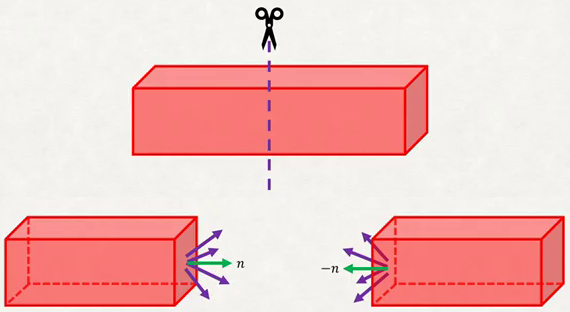
\includegraphics[width=20em]{phy_020_strs_02_01.png}

Kesit düzleminden bahsedelim önce, kesit tam dik olabilir ama bu şart değil,
nasıl olursa olsun o düzleme dik olan bir $\vec{n}$ vektörü ile bu kesitin
duruşunu temsil edebiliriz. 

Bu serbest bırakılmış iç kuvvetler darmadağın gözüküyor. Bir $\Delta A$
alanı tanımlayıp o alandaki tüm kuvvetleri alıp toplarsak bir $\Delta F$
elde edebiliriz, bu tek vektör daha derli toplu.

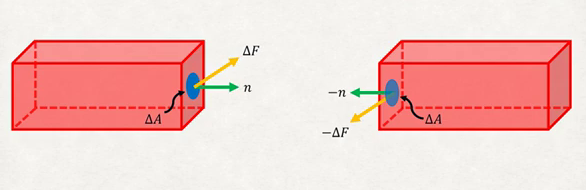
\includegraphics[width=20em]{phy_020_strs_02_02.png}

$\vec{n}$ ile tanımlı bir nokta etrafındaki düzlemin çekiş vektörünü (yani bir
noktadaki stres vektörü) şimdi şöyle tanımlıyoruz,

$$
t_n = \lim_{\Delta A \to 0} \frac{\Delta F}{\Delta A}
$$

Newton'un hareket kanunu üzerinden tabii ki sol taraftaki çekiş ile sağ
taraftaki birbirini dengelemeli, $t_n = -t_{-n}$.

Çekiş vektörü için formel tanım böyle. Ama kimse formel tanımı pek sevmiyor
sözel şekilde anlatırsak, çubuğu aldım ve kestim, Statik dersi der ki kaykılma
(shear), normal kuvvet ve eğilme momentimi böylece elde ederim. Bu üç boyutlu
nesnelerde olan şudur, çubuğu kesiyorum ve bileşenleri stres öğeleri olan tek
bir vektör elde ediyorum.

Şimdi çekiş vektörü kavramını daha basitleştirmeye uğraşalım. Bunun için
patatesimize geri dönüyoruz. Patatesten üç boyutlu sonsuz küçük küp şeklinde bir
parça çıkarttığımızı düşünelim şimdi,

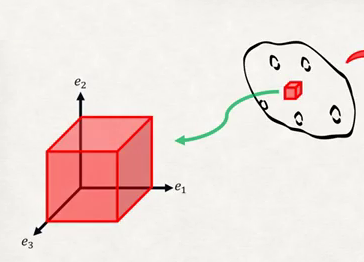
\includegraphics[width=15em]{phy_020_strs_02_03.png}

Bu ufak parça nesnenin bütünlüğünden çıkartıldığı için çekiş vektörlerinin
bu küpün yüzlerine etki eden stres vektörleri olduğunu söyleyebiliriz.

Küp sekli iyi bir seçim aslında çünkü her yüz kordinat eksendeki bir baz düzleme
paralel. Ayrıca $t_{e_1}$, $t_{e_2}$, $t_{e_3}$ yerine de daha iyi bir temsil
şekli bulabiliriz, küpün her yüzündeki bu $t$ çekiş vektörlerini de üç parçaya
ayırabiliriz,

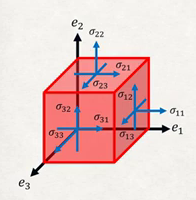
\includegraphics[width=10em]{phy_020_strs_02_04.png}

Bu sekildeki temsilin iyi bir tarafi her yuzdeki uc vektorun orijindeki
baz vektorlerle birebir uyusmasi. O zaman mesela $t_{e_3}$'u o baz vektorlerin
lineer bir kombinasyonu olarak yazabilirim,

$$
t_{e_3} = \sigma_{31} e_1 + \sigma_{32} e_2 + \sigma_{33} e_3
$$









[devam edecek]

\end{document}
